\newpage
\section*{Задание 6: Генерация синтетического датасета}
\subsection{Постановка задачи}
\noindent
Целевой класс объектов (для детекции): Спелые яблоки на дереве (АгроТех).\\
Базовое окружение (инвариант): Яблоневый сад.\\
Вариативные параметры (что менять в промпте): Сорт яблок (красные/зеленые), плотность листвы, солнечный свет.\\
Граничные случаи (сложные примеры): Гнилое яблоко, яблоко в тени листвы, гроздь яблок.\\
\newline
\indent
Необходимо сформировать синтетический датасет из 10–20 изображений, объединённых меткой «спелые яблоки на дереве», но отличающихся по условиям съёмки, сорту, освещению, ракурсу и наличию нестандартных ситуаций. Основная цель – продемонстрировать разнообразие выборки, достаточное для обучения модели компьютерного зрения (детекции объектов).
\newline
\subsection{Гипотеза и декомпозиция}
\indent Декомпозиция сцены: \\
Субъект: яблоки, спелые, красные, на ветке. \\
Окружение: яблоневый сад, листва.\\
Освещение: яркий солнечный свет, чёткие тени.\\
Стиль: фотореализм, высокая детализация.\\
Ракурс: по умолчанию – средний план.\\
\newpage
\indent Гипотеза: \\
добавление вариативных параметров (сорт, плотность листвы, освещение) и граничных случаев позволит получить разнообразные изображения, пригодные для обучения детектора. Косвенное управление через промпт (без явных параметров Seed/CFG) потребует уточняющих прилагательных и наречий для контроля степени детализации.
\subsection{Журнал генерации и отладки}
\indent \textbf{Итерация 1} \\
Промпт v1: \textit{«Спелые красные яблоки на дереве в яблоневом саду, солнечный день, фотореализм»} \\
\newline
Результат:
\begin{figure}[H]
	\centering
	
\includegraphics[width=17cm]{z6/1b.png}
	\caption{Итерация 1, модель (b)}
\end{figure}
\newpage
\begin{figure}[H]
	\centering
	
\includegraphics[width=15cm]{z6/1a.png}
	\caption{Итерация 1, модель (a)}
\end{figure}
\newpage
Изображение – ветка с несколькими крупными красными яблоками, яркий день, зелёные листья. Фон размыт. Яблоки имеют глянцевую поверхность, выглядят аппетитно.\\
\newline
\indent \textbf{Анализ ошибок:} \\
Яблоки только красные, сорт не варьируется.\\
Листва очень густая, что усложняет видимость плодов.\\
Освещение однотипное (яркое солнце).\\
Ракурс только один – крупный план. \\
\newline
\indent \textbf{Корректировка:} \\
Необходимо ввести переменные: указать возможность зелёных яблок, разную плотность листвы, другие условия освещения, ракурсы.\\
\newline
\indent \textbf{Итерация 2} \\
Промпт v2: \textit{«Спелые яблоки на дереве в яблоневом саду. Сорт яблок – смесь красных и зелёных. Листва средней густоты, видны ветки и плоды. Рассеянный свет, облачно. Фотореализм, средний план, высокая детализация»} \\
\newpage
Результат:
\begin{figure}[H]
	\centering
	
\includegraphics[width=14cm]{z6/2a.png}
	\caption{Итерация 2, модель (a)}
\end{figure}
\newpage
\begin{figure}[H]
	\centering
	
\includegraphics[width=17cm]{z6/2b.png}
	\caption{Итерация 2, модель (b)}
\end{figure}
На ветках видны и красные, и зелёные яблоки, листва не скрывает плоды. Освещение мягкое, без жёстких теней. Композиция – дерево в полроста. \\
\newline
\indent \textbf{Анализ ошибок:} \\
Не хватает разнообразия ракурсов (все изображения – средний план).
Отсутствуют граничные случаи (гниль, тень, гроздь).
Нет явного указания на разные сорта, модель сама выбирает оттенки. \\
% \newline
\indent \textbf{Корректировка:} \\
Добавим конкретные названия сортов, включим различные ракурсы (крупный план, общий вид, сверху вниз), введём граничные случаи. \\
\newline
\indent \textbf{Итерация 3} \\
Промпт v3 (шаблон): 
\textit{«Квадратное изображение. Спелые яблоки на дереве в яблоневом саду. Сорт: \{СОРТ\}. Листва: \{ГУСТОТА\}. Освещение: \{ОСВЕЩЕНИЕ\}. Ракурс: \{РАКУРС\}. Дополнительные особенности: \{ОСОБЕННОСТИ\}. Фотореализм, 8k, без водяных знаков»}
\newpage
\noindent
Подстановки для серии:
\begin{itemize}
	\item Сорта: «красные», «зелёные», «жёлто-красные».
	\item Густота листвы: «густая», «средняя», «редкая».
	\item Освещение: «яркое солнце, чёткие тени», «рассеянный свет, пасмурно», «контражур (солнце за спиной)».
	\item Ракурсы: «крупный план одной ветки», «общий план дерева», «вид снизу вверх», «вид сбоку».
	\item Особенности: «гнилое яблоко на ветке», «яблоко в тени листвы», «гроздь из трёх яблок».
\end{itemize}
\noindent
\newline
Примеры:
\begin{enumerate}
	\item Зелёные яблоки, редкая листва, рассеянный свет, общий план.
	\item Жёлто-красные яблоки, средняя листва, контражур, вид снизу.
	\item Гнилое яблоко (тёмное пятно) на ветке, остальные спелые, общий план.
	\item Яблоко в тени крупного листа, частично скрыто.
	\item Гроздь из трёх яблок на одной ветке, средний план.
\end{enumerate}
\newpage
\subsection{Визуализация результатов}
Наборы данных для генерации:
\begin{enumerate}
	\item Красные яблоки, густая листва, яркое солнце, крупный план
	\item Зелёные яблоки, редкая листва, контражур, вид снизу
	\item Зелёные яблоки, густая листва, пасмурно, средний план
	\item Жёлто-красные яблоки, средняя листва, яркое солнце, вид сбоку
	\item Гнилое яблоко (тёмное пятно) на ветке, остальные спелые, общий план
	\item Гнилое яблоко с морщинистой кожицей, крупный план
	\item Яблоко в тени листвы, частично скрыто, средний план
	\item Яблоко в тени, контражур, крупный план
	\item Гроздь из трёх яблок на одной ветке, средний план
\end{enumerate}
\newpage
Ниже представлена сетка 3x3, демонстрирующая 9 синтезированных изображений.
Они расположены в порядке возрастания от 1 до 9 (номер набора).
\begin{figure}[H]
	\centering
	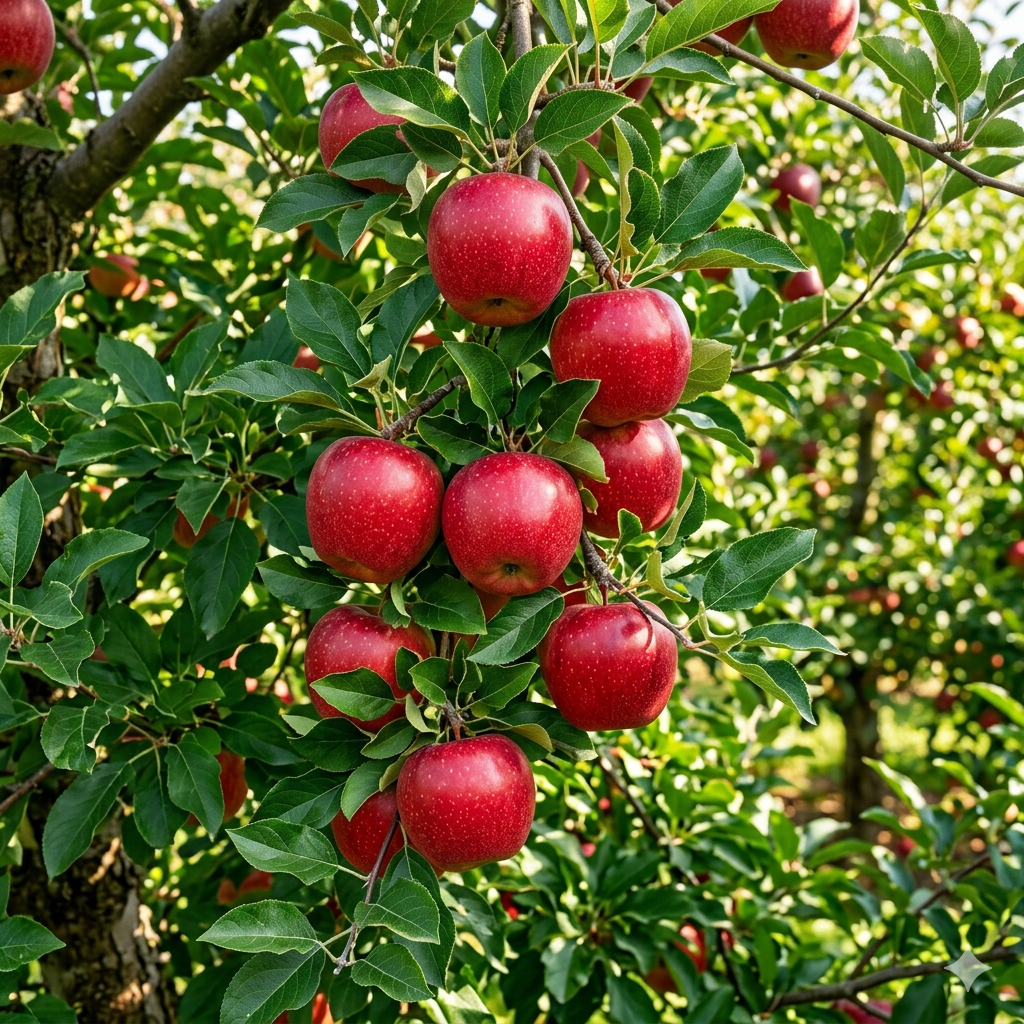
\includegraphics[width=5.6cm]{z6/3b1.png}
	\hfill
	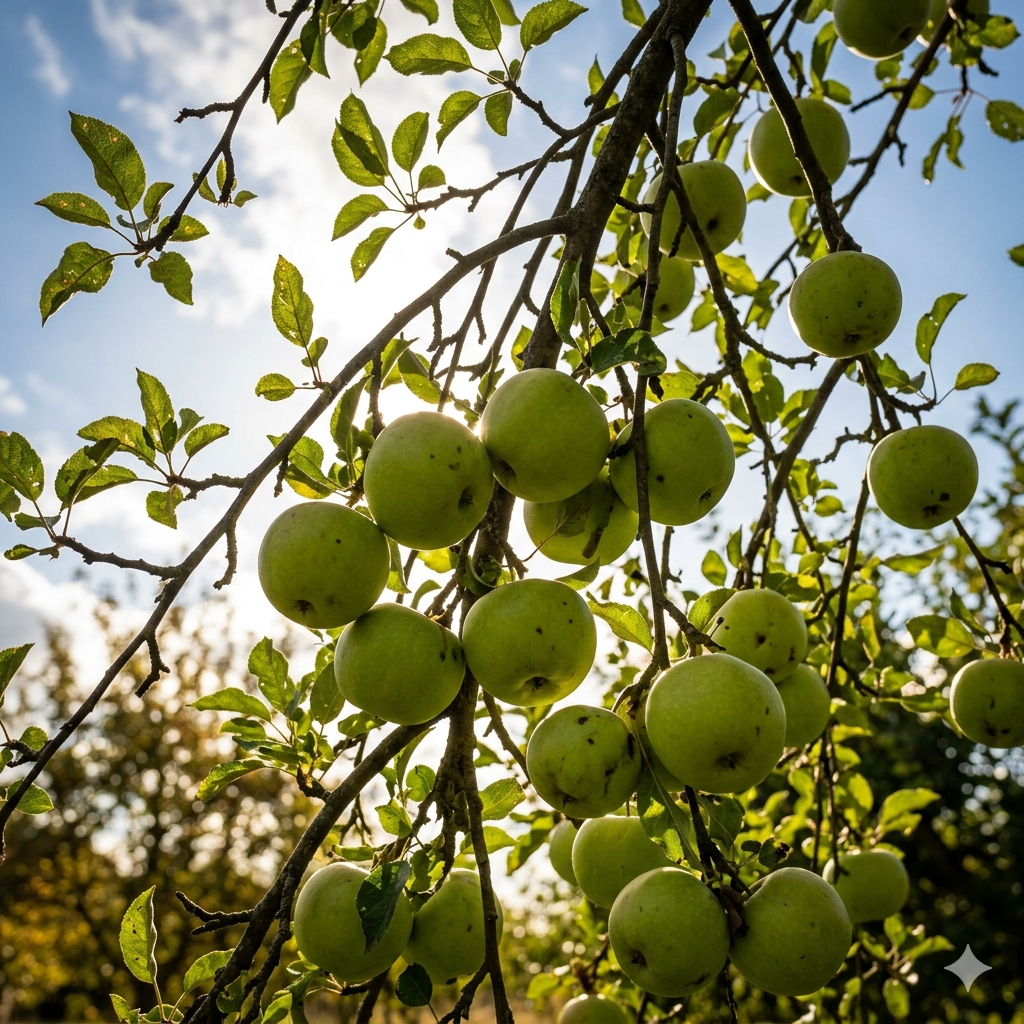
\includegraphics[width=5.6cm]{z6/3b2.png}
	\hfill
	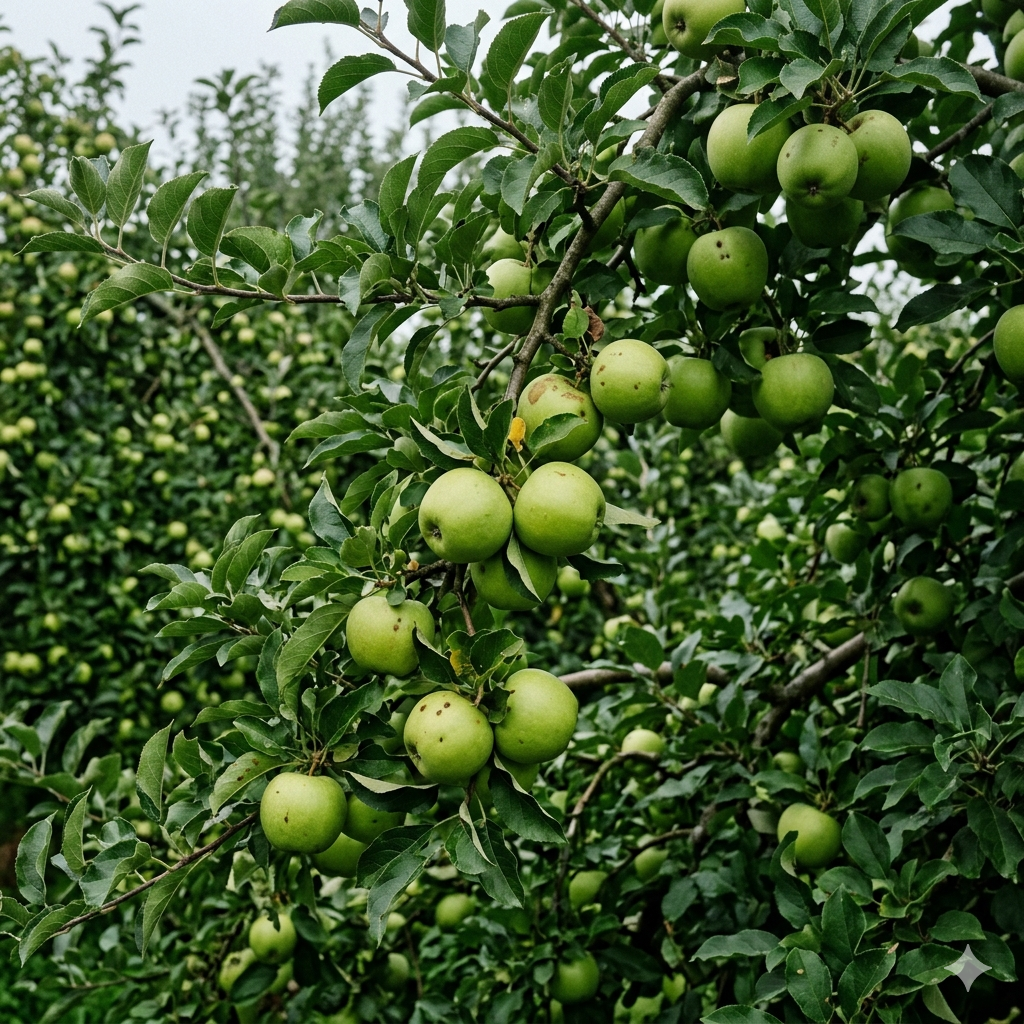
\includegraphics[width=5.6cm]{z6/3b3.png}
	% \caption{Референс и маска}
\end{figure}
\begin{figure}[H]
	\centering
	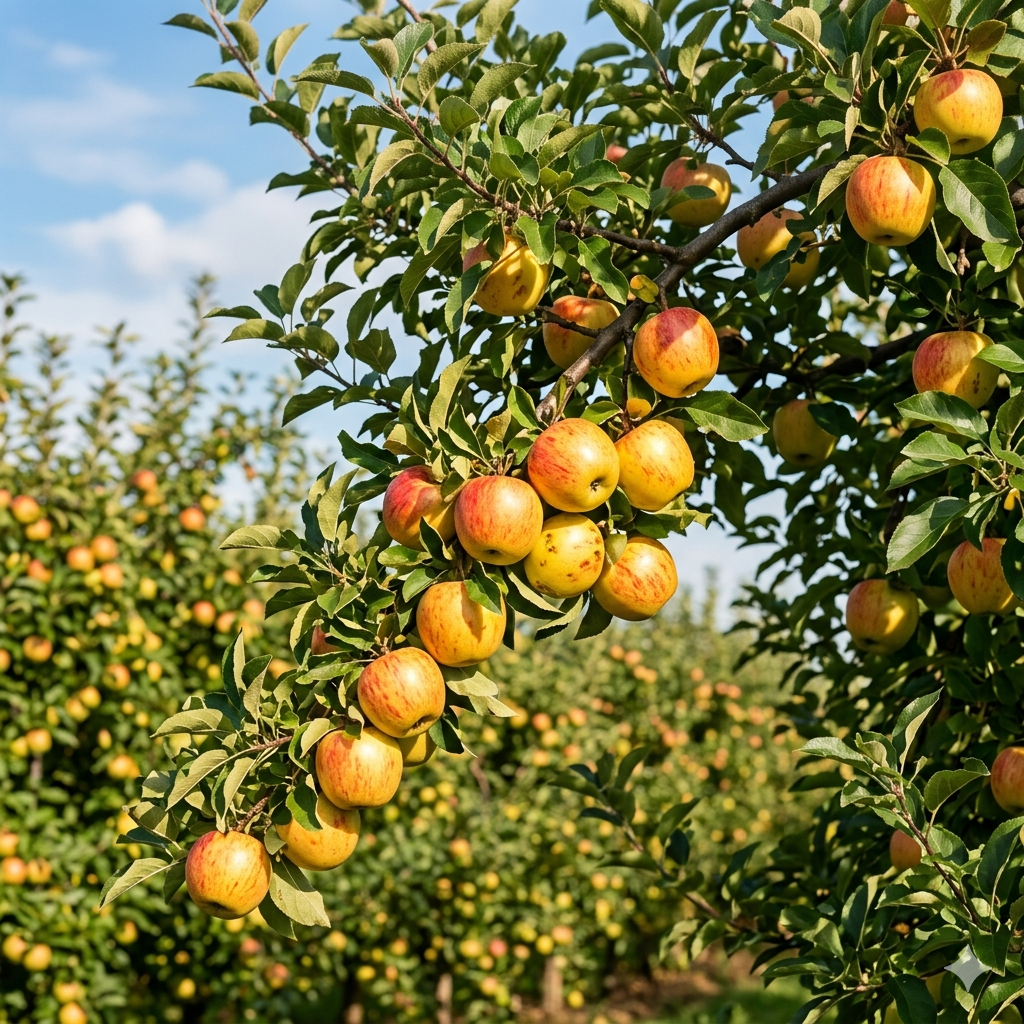
\includegraphics[width=5.6cm]{z6/3b4.png}
	\hfill
	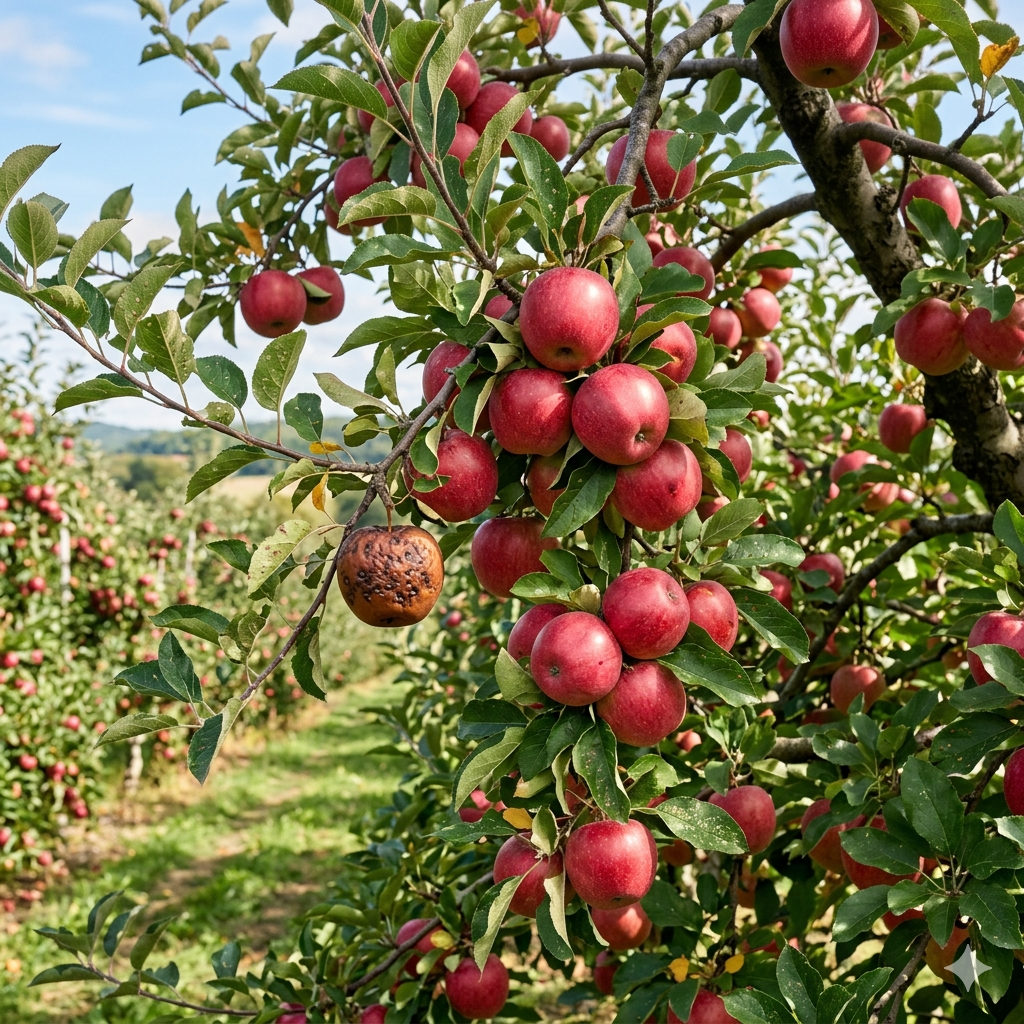
\includegraphics[width=5.6cm]{z6/3b5.png}
	\hfill
	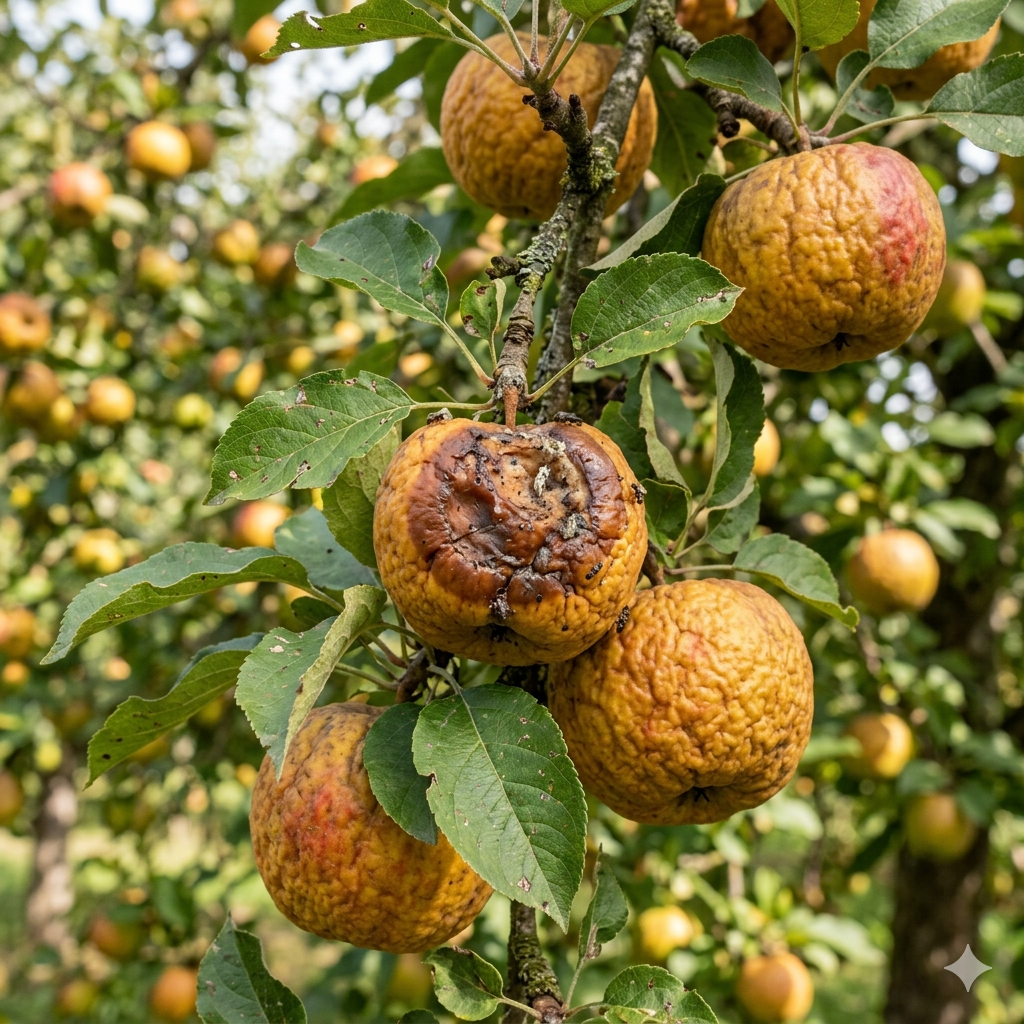
\includegraphics[width=5.6cm]{z6/3b6.png}
	% \caption{Референс и маска}
\end{figure}
\begin{figure}[H]
	\centering
	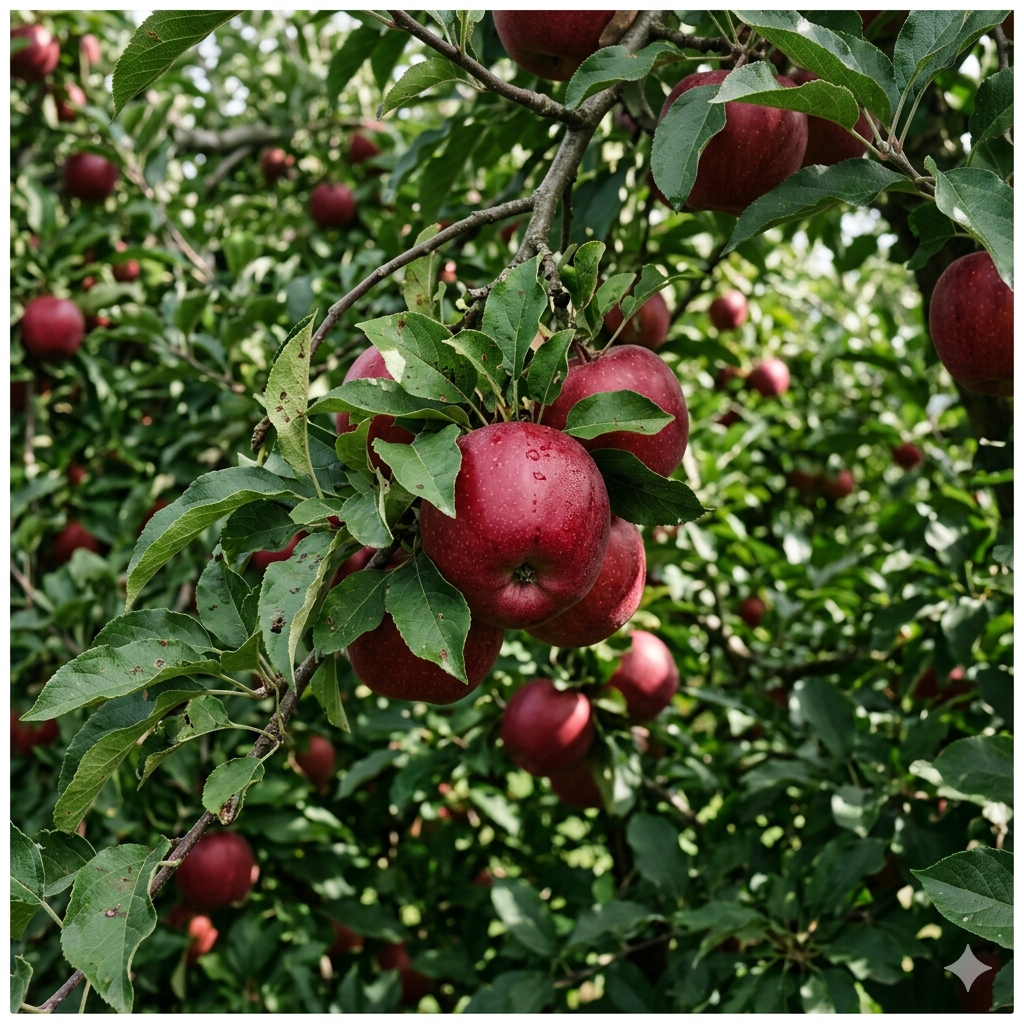
\includegraphics[width=5.6cm]{z6/3b7.png}
	\hfill
	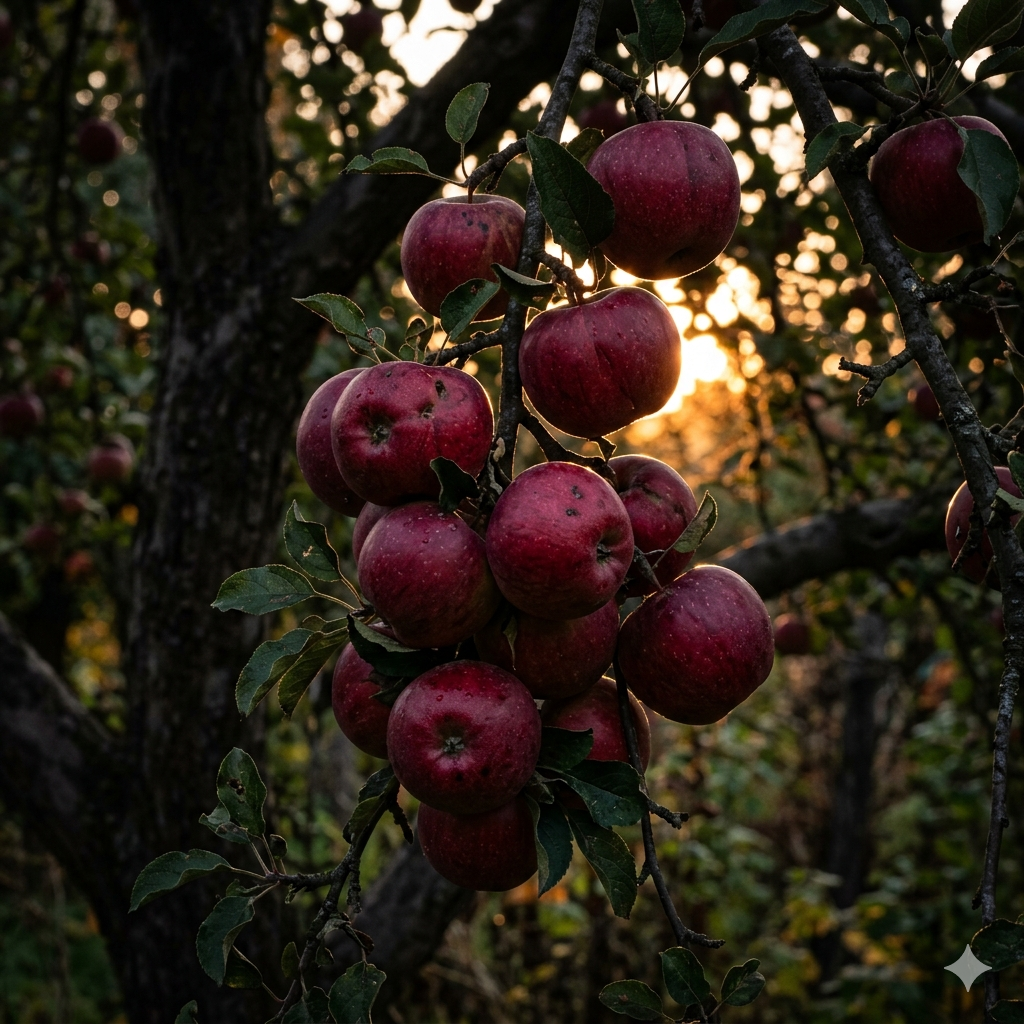
\includegraphics[width=5.6cm]{z6/3b8.png}
	\hfill
	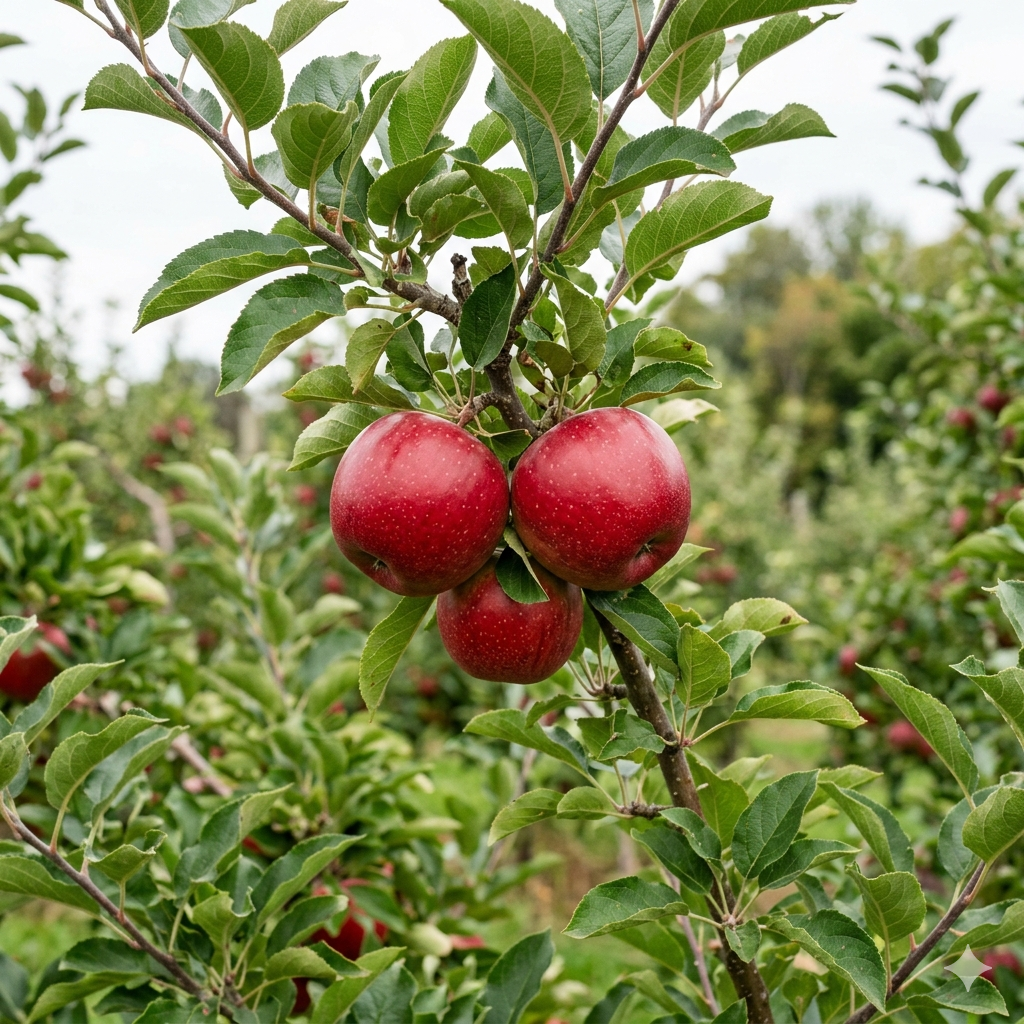
\includegraphics[width=5.6cm]{z6/3b9.png}
	% \caption{Референс и маска}
\end{figure}
Все изображения сгенерированны моделью (b) и соответствуют единому стилю «фотореализм», что позволяет использовать их как единый датасет.
\newpage
\subsection{Сравнение моделей}
\begin{table}[h!]
	\centering
	\begin{tabular}{|l|p{5cm}|p{5cm}|}
		\hline
		\textbf{Критерий} & \textbf{модель (a)} & \textbf{модель (b)} \\
		\hline
		Следование промпту & 5 & 5 \\
		\hline
		Качество деталей & 4 & 5 \\
		\hline
		Разнообразие вариаций & 5 & 5 \\
		\hline
		Отсутствие артефактов  & 4 & 5 \\
		\hline
		\textbf{Итог} & 4.5 & 5\\
		\hline
	\end{tabular}
\end{table}
Модель (b) обеспечивает более стабильное следование сложным промптам и лучше справляется с граничными случаями. Модель (a) требует более жёсткой формулировки и иногда добавляет артефакты, но в целом пригодна для генерации синтетических данных при доработке промпта.
\subsection{Финальный промпт}
Итоговый шаблон промпта (переменные части в фигурными скобками): \\
\textit{«Квадратное изображение. Спелые яблоки на дереве в яблоневом саду. Сорт: \{СОРТ\}. Листва: \{ГУСТОТА\}. Освещение: \{ОСВЕЩЕНИЕ\}. Ракурс: \{РАКУРС\}. Дополнительные особенности: \{ОСОБЕННОСТИ\}. Фотореализм, 8k, без водяных знаков»} \\
\newline
Использованные значения переменных: \\
\{СОРТ\} $\in$ \{«красные», «зелёные», «жёлто-красные»\} \\
\{ГУСТОТА\} $\in$ \{«густая», «средняя», «редкая»\}\\
\{ОСВЕЩЕНИЕ\} $\in$ \{«яркое солнце, чёткие тени», «рассеянный свет, пасмурно», «контражур (солнце за спиной)»\}\\
\{РАКУРС\} $\in$ \{«крупный план одной ветки», «общий план дерева», «вид снизу вверх», «вид сбоку»\}\\
\{ОСОБЕННОСТИ\} $\in$ \{«гнилое яблоко на ветке», «яблоко в тени листвы», «гроздь из трёх яблок»\}
\newpage
\subsection{Вывод}
\begin{enumerate}
	\item Разработанный шаблон промпта позволяет генерировать разнообразные синтетические изображения, покрывающие как типовые, так и граничные сценарии.
	\item Ключевыми факторами успеха стали: явное перечисление вариативных параметров, использование конкретных названий сортов и детализация освещения/ракурса.
	\item При отсутствии возможности управлять гиперпараметрами (Seed, CFG) косвенное управление через промпт (уточняющие прилагательные, перечисления) обеспечивает достаточный контроль над результатом.
	\item Сравнение моделей показало, что Модель (b) более предсказуема и точна для задачи генерации синтетических датасетов, что важно для инженерных приложений.
\end{enumerate}